\documentclass{beamer}
\usetheme{Madrid}
\usecolortheme{default}
\usepackage{tikz}
\usepackage{hyperref}

\title{Security Governance: Fundamentals and Best Practices}
\author{Instructor Name}
\institute{School/College Name}
\date{\today}

\begin{document}

\begin{frame}
\titlepage
\end{frame}

\begin{frame}
\frametitle{Introduction to Security Governance: Protecting What Matters}
\begin{itemize}
\item \textbf{Security governance} is the framework of rules, processes, and practices that ensure an organization protects its information assets.
\item Effective security governance aligns security practices with business objectives and stakeholder expectations.
\item Security governance establishes accountability and clear lines of responsibility for protecting systems and data.
\item Security governance reduces risks by providing structure and consistency to security efforts across an organization.
\end{itemize}

\begin{alertblock}{Why Security Governance Matters}
Without proper governance, security efforts become fragmented, inconsistent, and ineffective, leaving organizations vulnerable to threats.
\end{alertblock}
\end{frame}

\begin{frame}
\frametitle{The Security Governance Framework: An Overview}
\begin{columns}
\begin{column}{0.6\textwidth}
\begin{itemize}
\item A security governance framework provides the structure that guides all security decisions and activities.
\item The framework includes guidelines, policies, standards, and procedures that work together to protect assets.
\item Effective frameworks balance security needs with usability to avoid creating barriers to legitimate work.
\item Frameworks must adapt to changing threats, technologies, and regulatory requirements.
\end{itemize}
\end{column}
\begin{column}{0.4\textwidth}
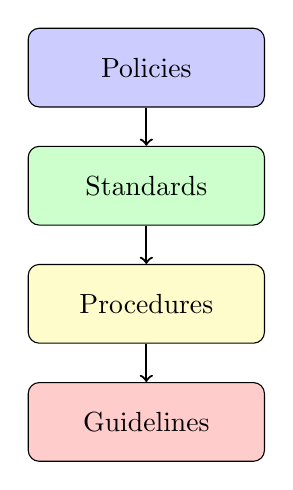
\begin{tikzpicture}[node distance=1.5cm]
\node (policies) [draw, rectangle, rounded corners, fill=blue!20, minimum width=3cm, minimum height=1cm] {Policies};
\node (standards) [draw, rectangle, rounded corners, fill=green!20, minimum width=3cm, minimum height=1cm, below of=policies] {Standards};
\node (procedures) [draw, rectangle, rounded corners, fill=yellow!20, minimum width=3cm, minimum height=1cm, below of=standards] {Procedures};
\node (guidelines) [draw, rectangle, rounded corners, fill=red!20, minimum width=3cm, minimum height=1cm, below of=procedures] {Guidelines};
\draw[->,thick] (policies) -- (standards);
\draw[->,thick] (standards) -- (procedures);
\draw[->,thick] (procedures) -- (guidelines);
\end{tikzpicture}
\end{column}
\end{columns}
\end{frame}

\begin{frame}
\frametitle{Security Guidelines: Setting the Foundation}
\begin{itemize}
\item \textbf{Security guidelines} are recommendations that suggest how security should be implemented without mandating specific actions.
\item Guidelines provide flexibility for different departments or situations while still promoting security best practices.
\item Guidelines often serve as the starting point for developing more specific security policies and standards.
\item Well-crafted guidelines help staff understand the reasoning behind security requirements.
\end{itemize}

\begin{exampleblock}{Example Guideline}
"Users should create passwords that are difficult for others to guess while still being memorable to themselves."
\end{exampleblock}
\end{frame}

\begin{frame}
\frametitle{Policy Development: Creating Clear Security Direction}
\begin{itemize}
\item \textbf{Security policies} are formal documents that define required behaviors, responsibilities, and consequences for non-compliance.
\item Effective policies clearly state what must be done rather than how it should be accomplished.
\item Policies should be written in clear, understandable language that avoids technical jargon when possible.
\item All security policies should be regularly reviewed and updated to address emerging threats and technologies.
\end{itemize}

\begin{block}{Policy Development Process}
\begin{enumerate}
\item Identify need and gather requirements
\item Draft policy with stakeholder input
\item Review and obtain approval
\item Communicate and implement
\item Monitor, enforce, and revise
\end{enumerate}
\end{block}
\end{frame}

\begin{frame}
\frametitle{Acceptable Use Policies (AUP): Defining Proper Technology Use}
\begin{itemize}
\item An \textbf{Acceptable Use Policy (AUP)} defines how employees may use company systems, networks, and data.
\item AUPs outline prohibited activities such as accessing inappropriate content or installing unauthorized software.
\item AUPs establish that company systems are primarily for business purposes and may be monitored.
\item Effective AUPs balance necessary restrictions with reasonable allowances for limited personal use.
\end{itemize}

\begin{table}
\small
\begin{tabular}{|p{5cm}|p{5cm}|}
\hline
\textbf{Typically Allowed} & \textbf{Typically Prohibited} \\
\hline
Limited personal email & Installing unauthorized software \\
Brief web browsing during breaks & Accessing inappropriate content \\
Occasional personal calls & Sharing credentials \\
Using approved cloud storage & Circumventing security controls \\
\hline
\end{tabular}
\caption{Common AUP Elements}
\end{table}
\end{frame}

\begin{frame}
\frametitle{Information Security Policies: Safeguarding Digital Assets}
\begin{itemize}
\item \textbf{Information security policies} establish rules for protecting the confidentiality, integrity, and availability of data.
\item These policies define data classification schemes that determine how different types of information should be handled.
\item Information security policies specify access control requirements based on the principle of least privilege.
\item They include requirements for data protection throughout its lifecycle, from creation to deletion.
\end{itemize}

\begin{block}{Key Information Security Policy Components}
\small
\begin{itemize}
\item Data classification (public, internal, confidential, restricted)
\item Access control requirements
\item Data handling procedures
\item Security incident reporting
\end{itemize}
\end{block}
\end{frame}

\begin{frame}
\frametitle{Business Continuity: Keeping Operations Running}
\begin{itemize}
\item \textbf{Business continuity} refers to maintaining essential functions during and after a disruptive event.
\item Business continuity policies define how an organization will continue operating during disasters, outages, or other crises.
\item These policies establish the maximum acceptable downtime for critical systems and processes.
\item Business continuity planning includes identifying essential functions and creating alternate procedures when normal operations are disrupted.
\end{itemize}

\begin{alertblock}{Business Impact Analysis (BIA)}
A BIA identifies critical business functions, determines the impact of disruptions, establishes recovery time objectives (RTOs), and informs resource allocation for continuity planning.
\end{alertblock}
\end{frame}

\begin{frame}
\frametitle{Disaster Recovery: Bouncing Back from Catastrophe}
\small
\begin{itemize}
\item \textbf{Disaster recovery} focuses specifically on restoring IT systems and infrastructure after a disruptive event.
\item Disaster recovery policies define the methods, tools, and procedures for recovering damaged systems.
\item These policies establish Recovery Time Objectives (RTO) and Recovery Point Objectives (RPO) for each system.
\item Effective disaster recovery requires regular testing, updating, and training for all involved personnel.
\end{itemize}

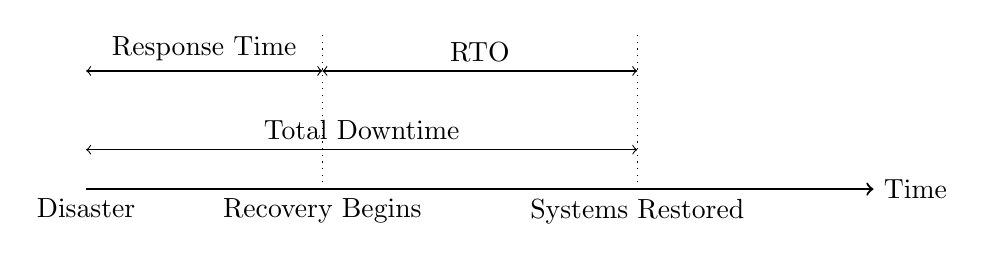
\begin{tikzpicture}
\draw[->,thick] (0,0) -- (10,0) node[right] {Time};
\draw (0,0) node[below] {Disaster};
\draw[dotted] (3,0) -- (3,2);
\draw (3,0) node[below] {Recovery Begins};
\draw[dotted] (7,0) -- (7,2);
\draw (7,0) node[below] {Systems Restored};
\draw[<->] (0,1.5) -- (3,1.5) node[midway,above] {Response Time};
\draw[<->] (3,1.5) -- (7,1.5) node[midway,above] {RTO};
\draw[<->] (0,0.5) -- (7,0.5) node[midway,above] {Total Downtime};
\end{tikzpicture}
\end{frame}


\begin{frame}
\frametitle{Incident Response: Managing Security Breaches}
\begin{itemize}
\item \textbf{Incident response} is the organized approach to addressing and managing security breaches.
\item Incident response policies define what constitutes a security incident and establish procedures for handling various types of incidents.
\item These policies create a structured framework that enables quick and effective responses to minimize damage.
\item Incident response requires clear communication protocols and defined roles for all team members.
\end{itemize}

\begin{block}{The Incident Response Lifecycle}
\scriptsize
\begin{enumerate}
\item Preparation: Create plans and train teams
\item Detection \& Analysis: Identify and assess the incident
\item Containment: Prevent the incident from spreading
\item Eradication: Remove the threat from systems
\item Recovery: Restore systems to normal operation
\item Lessons Learned: Improve future responses
\end{enumerate}
\end{block}
\end{frame}

\begin{frame}
\frametitle{SDLC Security: Building Safety into Software Development}
\begin{itemize}
\item \textbf{Software Development Lifecycle (SDLC)} security integrates security practices throughout the entire development process.
\item SDLC security policies establish requirements for secure coding, testing, and validation at each development phase.
\item These policies mandate security reviews and testing before software can move to the next development stage.
\item Effective SDLC security shifts the focus from fixing vulnerabilities after deployment to preventing them during development.
\end{itemize}

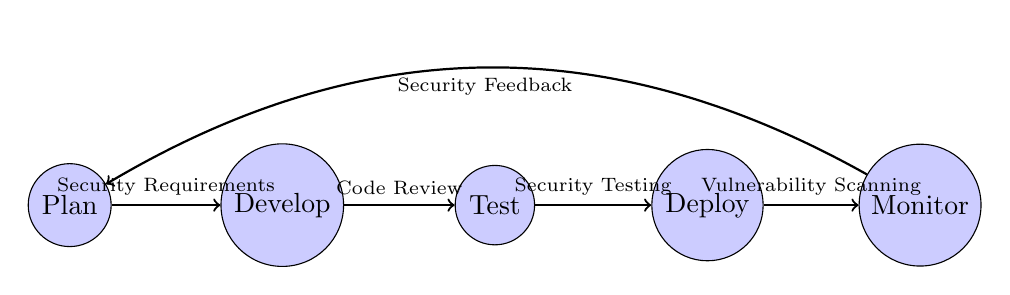
\begin{tikzpicture}[node distance=1.2cm]
\node (plan) [draw, circle, fill=blue!20] {Plan};
\node (develop) [draw, circle, fill=blue!20, right of=plan, xshift=1.5cm] {Develop};
\node (test) [draw, circle, fill=blue!20, right of=develop, xshift=1.5cm] {Test};
\node (deploy) [draw, circle, fill=blue!20, right of=test, xshift=1.5cm] {Deploy};
\node (monitor) [draw, circle, fill=blue!20, right of=deploy, xshift=1.5cm] {Monitor};

\draw[->,thick] (plan) -- node[above] {\scriptsize Security Requirements} (develop);
\draw[->,thick] (develop) -- node[above] {\scriptsize Code Review} (test);
\draw[->,thick] (test) -- node[above] {\scriptsize Security Testing} (deploy);
\draw[->,thick] (deploy) -- node[above] {\scriptsize Vulnerability Scanning} (monitor);
\draw[->,thick, bend right] (monitor) to node[below] {\scriptsize Security Feedback} (plan);
\end{tikzpicture}
\end{frame}

\begin{frame}
\frametitle{Change Management Policies: Controlling System Modifications}
\begin{itemize}
\item \textbf{Change management policies} establish processes for making changes to IT systems in a controlled, documented manner.
\item These policies require formal approval processes before changes can be implemented in production environments.
\item Change management ensures that modifications are properly tested and do not negatively impact security or functionality.
\item Effective change management includes rollback plans in case changes create unexpected problems.
\end{itemize}

\begin{exampleblock}{Example Change Management Process}
\scriptsize
A system administrator wants to update server software. They must:
\begin{enumerate}
\item Submit a change request with details and justification
\item Obtain approval from the change advisory board
\item Schedule the change during an approved maintenance window
\item Test the change in a non-production environment first
\item Document results and follow rollback procedures if needed
\end{enumerate}
\end{exampleblock}
\end{frame}

\begin{frame}
\frametitle{Security Standards: Establishing Consistent Practices}
\begin{itemize}
\item \textbf{Security standards} define specific, mandatory requirements for implementing security controls.
\item Standards provide detailed technical specifications that support the broader objectives stated in security policies.
\item Unlike guidelines, standards leave little room for interpretation and establish clear compliance requirements.
\item Effective standards balance security needs with practicality to ensure they can be reasonably implemented.
\end{itemize}

\begin{table}
\small
\begin{tabular}{|p{3.5cm}|p{7cm}|}
\hline
\textbf{Security Element} & \textbf{Example Standard Requirement} \\
\hline
Passwords & Minimum 12 characters with complexity requirements \\
\hline
System Updates & Critical patches must be applied within 14 days \\
\hline
Data Encryption & All sensitive data must use AES-256 encryption \\
\hline
Access Reviews & Administrator access must be reviewed quarterly \\
\hline
\end{tabular}
\caption{Example Security Standards}
\end{table}
\end{frame}


\begin{frame}
\frametitle{Password Standards: Creating Strong Authentication Rules}
\begin{itemize}
\item \textbf{Password standards} define specific requirements for creating, managing, and protecting user credentials.
\item These standards specify minimum password length, complexity requirements, and expiration periods.
\item Password standards often include rules for password storage, such as requiring salted hashing rather than storing plaintext passwords.
\item Effective standards balance security needs with usability to avoid encouraging risky workarounds like writing passwords down.
\end{itemize}

\begin{alertblock}{Modern Password Guidance}
\scriptsize
The National Institute of Standards and Technology (NIST) now recommends:
\begin{itemize}
\item Longer passwords (at least 12 characters)
\item Checking new passwords against lists of commonly used or compromised passwords
\item Eliminating arbitrary complexity requirements
\item Removing periodic password change requirements
\end{itemize}
\end{alertblock}
\end{frame}

\begin{frame}
\frametitle{Access Control Standards: Managing Who Gets In}
\begin{itemize}
\item \textbf{Access control standards} define requirements for granting, managing, and revoking access to systems and data.
\item These standards implement the principle of least privilege, ensuring users have only the access necessary for their job functions.
\item Access control standards require regular reviews of user permissions to identify and remove unnecessary access rights.
\item Effective standards include special provisions for privileged accounts that have elevated system access.
\end{itemize}

\begin{table}
\scriptsize
\centering
\begin{tabular}{|c|c|}
\hline
\textbf{Control Type} & \textbf{Examples} \\
\hline
Preventive Controls & \begin{tabular}{@{}c@{}}
Authentication \\
Authorization
\end{tabular} \\
\hline
Detective Controls & \begin{tabular}{@{}c@{}}
Access auditing \\
Login monitoring
\end{tabular} \\
\hline
Corrective Controls & \begin{tabular}{@{}c@{}}
Account lockout \\
Password reset
\end{tabular} \\
\hline
Compensating Controls & \begin{tabular}{@{}c@{}}
Multi-factor authentication \\
Separation of duties
\end{tabular} \\
\hline
\end{tabular}
\caption{Examples of Access Control Standards}
\end{table}
\end{frame}

\begin{frame}
\frametitle{Physical Security Standards: Protecting Tangible Assets}
\begin{itemize}
\item \textbf{Physical security standards} establish requirements for protecting facilities, equipment, and physical information assets.
\item These standards define access requirements for different security zones within facilities (e.g., lobbies, server rooms).
\item Physical security standards include requirements for monitoring systems like cameras and intrusion detection.
\item Effective standards consider both deliberate threats (theft, vandalism) and environmental risks (fire, flood, power loss).
\end{itemize}

\begin{exampleblock}{Example: Server Room Requirements}
\scriptsize
\begin{itemize}
\item Access limited to authorized IT personnel via card readers with PIN
\item 24/7 video surveillance with 90-day retention
\item Environmental monitoring for temperature, humidity, and water
\item Fire suppression system specific to electronic equipment
\end{itemize}
\end{exampleblock}
\end{frame}

\begin{frame}
\frametitle{Encryption Standards: Securing Data Transmission and Storage}
\begin{itemize}
\item \textbf{Encryption standards} define requirements for protecting data confidentiality through cryptographic methods.
\item These standards specify which encryption algorithms and key lengths must be used for different types of data.
\item Encryption standards establish requirements for key management, including generation, storage, and rotation practices.
\item Effective standards address both data at rest (stored) and data in transit (being transmitted).
\end{itemize}

\begin{table}
\scriptsize
\begin{tabular}{|p{2.5cm}|p{3cm}|p{3.5cm}|}
\hline
\textbf{Data Type} & \textbf{Encryption Method} & \textbf{Key Management} \\
\hline
Data at rest & AES-256 & Keys stored in secure hardware \\
\hline
Data in transit & TLS 1.3 & Certificates rotated annually \\
\hline
Emails & S/MIME or PGP & Key pairs for each user \\
\hline
Backups & AES-256 & Offline key storage \\
\hline
\end{tabular}
\caption{Example Encryption Standards}
\end{table}
\end{frame}

\begin{frame}
\frametitle{Security Procedures: Implementing Day-to-Day Practices}
\begin{itemize}
\item \textbf{Security procedures} are detailed, step-by-step instructions for performing specific security-related tasks.
\item Procedures translate high-level policies and standards into practical, actionable steps for implementation.
\item Well-written procedures reduce human error by providing clear guidance for complex or infrequent tasks.
\item Effective procedures include verification steps to confirm proper completion and documentation requirements.
\end{itemize}

\begin{block}{Components of Effective Security Procedures}
\scriptsize
\begin{itemize}
\item Clear purpose and scope statement
\item Required tools and prerequisites
\item Detailed sequential steps with screenshots or diagrams
\item Expected outcomes and verification methods
\item Troubleshooting guidance for common issues
\end{itemize}
\end{block}
\end{frame}

\begin{frame}
\frametitle{Change Management Procedures: Steps for Safe System Updates}
\begin{itemize}
\item \textbf{Change management procedures} provide detailed instructions for implementing the change management policy.
\item These procedures define the exact steps for requesting, approving, implementing, and documenting changes.
\item Change management procedures include methods for categorizing changes based on risk and potential impact.
\item Effective procedures establish different approval paths for routine, significant, and emergency changes.
\end{itemize}

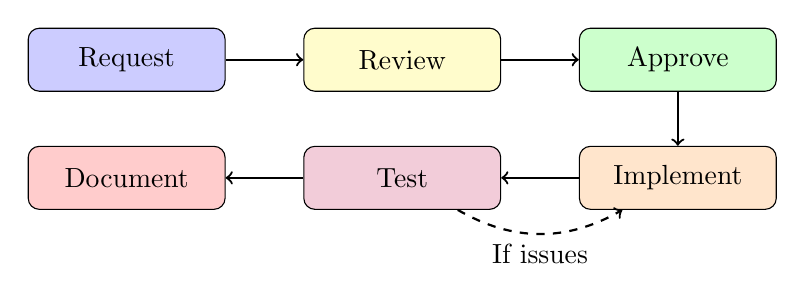
\begin{tikzpicture}[node distance=1.5cm]
\node (request) [draw, rectangle, rounded corners, fill=blue!20, minimum width=2.5cm, minimum height=0.8cm] {Request};
\node (review) [draw, rectangle, rounded corners, fill=yellow!20, minimum width=2.5cm, minimum height=0.8cm, right of=request, xshift=2cm] {Review};
\node (approve) [draw, rectangle, rounded corners, fill=green!20, minimum width=2.5cm, minimum height=0.8cm, right of=review, xshift=2cm] {Approve};
\node (implement) [draw, rectangle, rounded corners, fill=orange!20, minimum width=2.5cm, minimum height=0.8cm, below of=approve] {Implement};
\node (test) [draw, rectangle, rounded corners, fill=purple!20, minimum width=2.5cm, minimum height=0.8cm, left of=implement, xshift=-2cm] {Test};
\node (document) [draw, rectangle, rounded corners, fill=red!20, minimum width=2.5cm, minimum height=0.8cm, left of=test, xshift=-2cm] {Document};

\draw[->,thick] (request) -- (review);
\draw[->,thick] (review) -- (approve);
\draw[->,thick] (approve) -- (implement);
\draw[->,thick] (implement) -- (test);
\draw[->,thick] (test) -- (document);
\draw[->,thick,dashed] (test) to[bend right] node[below] {If issues} (implement);
\end{tikzpicture}
\end{frame}

\begin{frame}
\frametitle{Onboarding Procedures: Securely Adding New Users}
\begin{itemize}
\item \textbf{Onboarding procedures} define the process for granting new employees appropriate access to systems and data.
\item These procedures establish verification requirements to confirm user identity before access is granted.
\item Onboarding procedures include security training requirements that must be completed before users receive full access.
\item Effective onboarding creates a complete record of all access granted for future reference and auditing.
\end{itemize}

\begin{exampleblock}{Sample Onboarding Procedure Steps}
\scriptsize
\begin{enumerate}
\item HR verifies employee identity and provides documented approval
\item IT creates accounts based on role-specific access templates
\item Employee completes security awareness training
\item Employee acknowledges acceptance of security policies
\item Manager confirms appropriate access levels
\item Access provisioning is documented in access management system
\end{enumerate}
\end{exampleblock}
\end{frame}

\begin{frame}
\frametitle{Offboarding Procedures: Safely Removing Access}
\begin{itemize}
\item \textbf{Offboarding procedures} define the process for removing access when an employee leaves the organization.
\item These procedures establish timelines for access removal based on the nature of the departure (e.g., immediate for terminations, phased for retirements).
\item Offboarding procedures include steps to recover company equipment and data from departing employees.
\item Effective offboarding requires coordination between HR, IT, facilities, and the employee's department.
\end{itemize}

\begin{table}
\scriptsize
\begin{tabular}{|p{3cm}|p{3cm}|p{3cm}|}
\hline
\textbf{Departure Type} & \textbf{Access Removal Timeline} & \textbf{Special Considerations} \\
\hline
Voluntary resignation & End of last workday & Knowledge transfer period \\
\hline
Retirement & End of last workday & Phased transition period \\
\hline
Termination & Immediate & Monitor final access activities \\
\hline
Transfer & Based on new role start & Modify rather than remove \\
\hline
\end{tabular}
\caption{Offboarding Timeline Examples}
\end{table}
\end{frame}

\begin{frame}
\frametitle{Security Playbooks: Standardized Response Actions}
\begin{itemize}
\item \textbf{Security playbooks} are detailed action plans for responding to specific security incidents or scenarios.
\item Playbooks provide step-by-step instructions that reduce decision-making burden during high-stress situations.
\item Well-designed playbooks include decision trees to guide responders through different scenario variations.
\item Effective playbooks assign clear responsibilities to specific roles rather than individuals to ensure coverage.
\end{itemize}

\begin{block}{Common Security Playbook Elements}
\scriptsize
\begin{itemize}
\item Incident identification criteria and severity classifications
\item Required tools and resources for response
\item Communication templates and escalation paths
\item Detailed containment and eradication steps
\item Evidence collection and preservation procedures
\item Recovery validation checkpoints
\end{itemize}
\end{block}
\end{frame}

\begin{frame}
\frametitle{External Regulatory Considerations: Compliance Requirements}
\begin{itemize}
\item \textbf{Regulatory compliance} involves adhering to laws, regulations, and standards established by external authorities.
\item Security governance must account for industry-specific regulations that mandate certain security controls or practices.
\item Non-compliance with regulations can result in significant financial penalties, legal liability, and reputational damage.
\item Effective governance includes monitoring regulatory changes to ensure continued compliance as requirements evolve.
\end{itemize}

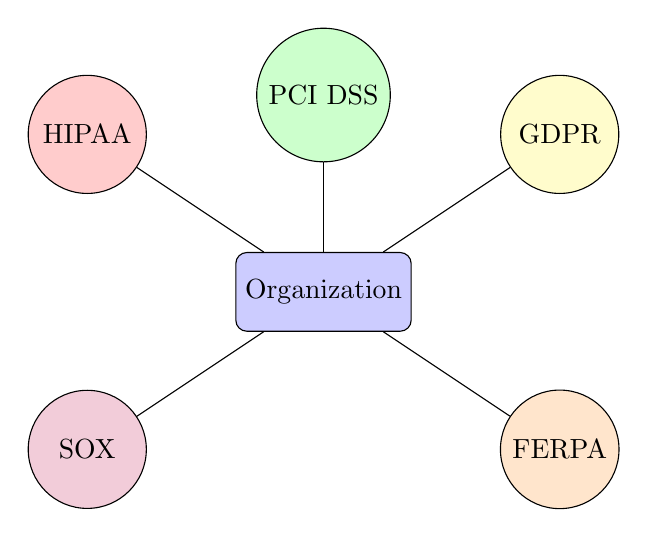
\begin{tikzpicture}
\node[draw, rectangle, rounded corners, minimum width=2cm, minimum height=1cm, fill=blue!20] (org) at (0,0) {Organization};

\node[draw, circle, minimum width=1.5cm, fill=red!20] (hipaa) at (-3,2) {HIPAA};
\node[draw, circle, minimum width=1.5cm, fill=green!20] (pci) at (0,2.5) {PCI DSS};
\node[draw, circle, minimum width=1.5cm, fill=yellow!20] (gdpr) at (3,2) {GDPR};
\node[draw, circle, minimum width=1.5cm, fill=purple!20] (sox) at (-3,-2) {SOX};
\node[draw, circle, minimum width=1.5cm, fill=orange!20] (ferpa) at (3,-2) {FERPA};

\draw[-] (org) -- (hipaa);
\draw[-] (org) -- (pci);
\draw[-] (org) -- (gdpr);
\draw[-] (org) -- (sox);
\draw[-] (org) -- (ferpa);
\end{tikzpicture}
\end{frame}

\begin{frame}
\frametitle{Legal Considerations in Security Governance}
\begin{itemize}
\item Security governance must align with relevant laws regarding data protection, privacy, and breach notification.
\item Legal considerations include liability for security failures that impact customers, partners, or the public.
\item Security governance documentation may become legal evidence during investigations or litigation.
\item Effective governance includes consultation with legal experts when developing policies for sensitive areas.
\end{itemize}

\begin{alertblock}{Legal Compliance Considerations}
\scriptsize
\begin{itemize}
\item Data breach notification requirements vary by jurisdiction
\item Privacy laws restrict how personal data can be collected and used
\item Contractual obligations may impose additional security requirements
\item Intellectual property laws affect how proprietary information must be protected
\end{itemize}
\end{alertblock}
\end{frame}

\begin{frame}
\frametitle{Industry-Specific Security Standards}
\begin{itemize}
\item \textbf{Industry-specific security standards} are frameworks tailored to address unique risks in particular sectors.
\item These standards often develop through industry associations or specialized regulatory bodies.
\item Industry standards may be voluntary but can become de facto requirements for doing business in certain sectors.
\item Effective governance leverages these standards to establish baseline security controls relevant to the organization's industry.
\end{itemize}

\begin{table}
\scriptsize
\begin{tabular}{|p{2.5cm}|p{3cm}|p{4cm}|}
\hline
\textbf{Industry} & \textbf{Standard} & \textbf{Focus Areas} \\
\hline
Healthcare & HIPAA & Patient data privacy and security \\
\hline
Financial & PCI DSS & Payment card processing security \\
\hline
Critical Infrastructure & NERC CIP & Power grid protection \\
\hline
Government & FedRAMP & Cloud service security \\
\hline
\end{tabular}
\caption{Example Industry Standards}
\end{table}
\end{frame}


\begin{frame}
\frametitle{Local and Regional Security Regulations}
\begin{itemize}
\item \textbf{Local and regional regulations} establish security and privacy requirements specific to geographic areas.
\item These regulations can vary significantly between different cities, states, provinces, or regions.
\item Organizations operating in multiple locations must ensure compliance with all applicable local requirements.
\item Effective governance includes monitoring for new or changing local regulations that may impact security practices.
\end{itemize}

\begin{exampleblock}{Examples of Regional Security Regulations}
    \scriptsize
\begin{itemize}
\item California Consumer Privacy Act (CCPA) applies specifically to businesses operating in California
\item New York SHIELD Act establishes specific data security requirements for companies with New York residents' data
\item Illinois Biometric Information Privacy Act (BIPA) regulates collection and storage of biometric data
\item Massachusetts 201 CMR 17.00 establishes specific technical security requirements for personal information
\end{itemize}
\end{exampleblock}
\end{frame}

\begin{frame}
\frametitle{National Security Standards and Laws}
\begin{itemize}
\item \textbf{National security standards} provide frameworks that apply to all organizations within a country.
\item These standards establish baseline security expectations that may be further strengthened by industry regulations.
\item National laws often include penalties for security breaches or failure to implement reasonable security measures.
\item Effective governance ensures compliance with both mandatory requirements and voluntary national standards.
\end{itemize}

\begin{table}
    \scriptsize
\begin{tabular}{|p{3cm}|p{3cm}|p{3cm}|}
\hline
\textbf{Country} & \textbf{Standard/Law} & \textbf{Primary Focus} \\
\hline
United States & FISMA & Federal information security \\
\hline
United Kingdom & Data Protection Act & Personal data protection \\
\hline
Australia & Privacy Act & Data breach notification \\
\hline
Canada & PIPEDA & Consumer privacy \\
\hline
\end{tabular}
\caption{National Security Standards Examples}
\end{table}
\end{frame}

\begin{frame}
\frametitle{Global Security Frameworks and Regulations}
\begin{itemize}
\item \textbf{Global security frameworks} provide standardized approaches recognized across international boundaries.
\item These frameworks help organizations establish security governance that satisfies requirements in multiple countries.
\item Global regulations like GDPR may apply to organizations regardless of where they are physically located.
\item Effective governance identifies which global frameworks best align with the organization's operations and compliance needs.
\end{itemize}

\begin{block}{Key Global Security Frameworks}
    \scriptsize
\begin{itemize}
\item \textbf{ISO 27001}: International standard for information security management systems
\item \textbf{NIST Cybersecurity Framework}: Flexible framework for managing and reducing cybersecurity risk
\item \textbf{CIS Controls}: Prioritized set of actions to protect critical systems and data
\item \textbf{COBIT}: Framework for governance and management of enterprise information technology
\end{itemize}
\end{block}
\end{frame}

\begin{frame}
\frametitle{Monitoring and Revising Security Governance}
\begin{itemize}
\item \textbf{Security governance monitoring} involves regular assessment of how well policies and standards are being followed.
\item Effective governance requires continuous review to address emerging threats, technologies, and regulatory changes.
\item Revisions should be based on compliance data, incident response lessons, and security testing results.
\item A formal review cycle ensures all governance documents remain relevant and effective over time.
\end{itemize}

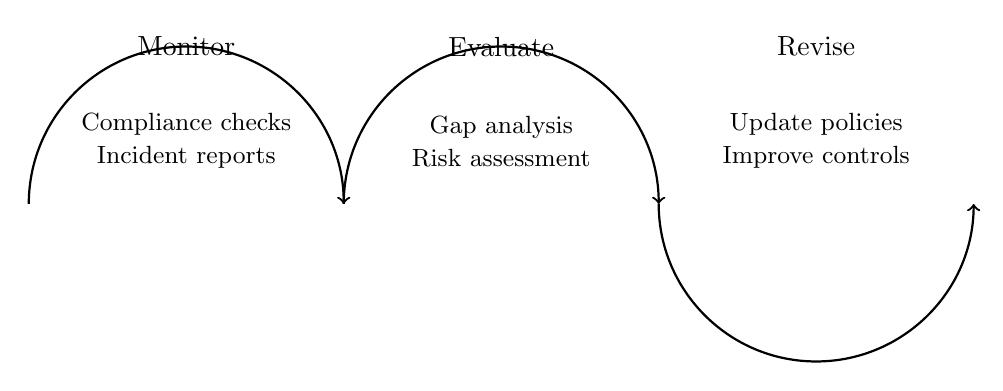
\begin{tikzpicture}
\draw[->,thick] (0,0) arc (180:0:2);
\draw[->,thick] (4,0) arc (180:0:2);
\draw[->,thick] (8,0) arc (180:360:2);

\node at (2,2) {Monitor};
\node at (6,2) {Evaluate};
\node at (10,2) {Revise};

\node[align=center] at (2,0.8) {\small Compliance checks\\\small Incident reports};
\node[align=center] at (6,0.8) {\small Gap analysis\\\small Risk assessment};
\node[align=center] at (10,0.8) {\small Update policies\\\small Improve controls};
\end{tikzpicture}
\end{frame}
\end{document}